\chapter{Analise Sobre Abstrações de Processos}
\label{cap:analise-sobre-abstracoes-de-processos}

No Capítulo \ref{cap:trabalhos-analisados} introduzimos os principais trabalhos
que orbitam sobre o tema de novas abstrações de processos para que nesse
capítulo seja feito uma reflexão cuidadosa sobre as principais características
dos mesmos. Durante o capítulo realizamos diversas analises sobre o estado da
arte dos diferentes trabalhos e apresentamos um modelo teórico que visa
apresentar uma perspectiva para a nova geração de abstrações de processos. Esse
capítulo responde as seguintes perguntas de pesquisa:

\begin{quote}
 \item \textit{RQ1:.} "Quais são as características desejáveis para a próxima geração de abstração de processos?"
 \item \textit{RQ2:.} "Quais são os principais desafios em se implementar a próxima geração de abstração de processos?"
\end{quote}


\section{Potenciais e dificuldades para adotar novas abstrações de processos}
\label{sec:potenciais}

Pesquisas em SO buscam avançar o estado da arte desse campo, contudo, SOs
usados em produção e projetos de pesquisa tem diferentes restrições. Se uma
nova proposta feita pela academia tem por objetivo ser utilizada em aplicações
que estão no estado da prática, essas devem considerar questões referentes
a compatibilidade, melhor uso do hardware atual, confiabilidade e ser genérico
o bastante para ser utilizado por múltiplas linguagens de programação.

Os SOs usados em produção demandam uma rigorosa validação para manter o sistema
estável em uma variedade de configurações, como prevenir acesso ilegal a
memória, impossibilitar violação de API, evitar consumo excessivo de recursos e
impedir erros de sincronização ou \textit{locking}. Essas características tem
que ser garantidas pelo SO \citep{mondrix}, como pode-se esperar, tais
restrições são complicadas de atendidas por propostas de pesquisas que
normalmente concentram-se em um único problema sem considerar outros impactos.
Por esses motivos, para que um novo componente sugerido por meio de pesquisa
atinga os SOs atuais, é importante garantir fique as aplicações que já existem
não sofram impactos negativos em termos de desempenho e de uso.

Outra perspectiva a se considerar é o contínuo desenvolvimento de novos
recursos no nível do hardware, por exemplo, é comum observar componentes que
são especializados em um nicho e que ao longo do tempo chegam ao usuário
final tornando-se comum. Um caso simples que ilustra tal evolução é o
uso de hardware especializado para virtualização, uma vez que esses existiam
apenas para servidores e hoje estão disponíveis para a maioria dos usuários
comuns. Tais recursos representam um novo leque de opções não exploradas,
inclusive para trazer melhorias para as atuais abstrações de processos.
Entretanto, qualquer tentativa de incorporar os novos recursos de hardware para
a abstração de processos deve levar em consideração que alguns usuários podem
não ter tal recurso disponível. Por essa razão qualquer mudança nos processos
que adicionem suporte a novos recursos de hardware devem levar em consideração
todo tipo de caso. De modo inverso, propostas para melhorar uma abstração de
processos podem sugerir mudanças para hardware sendo útil para avançar os
estado da arte dos chips modernos. Claro que a evolução do hardware deve ter
cuidado para não quebrar a compatibilidade binária com aplicações legadas.
Infelizmente, é preciso ter em mente que tais limitações fazem com que a ampla
adoção de uma determinada melhoria seja impraticável.

Algumas das novas abstrações de processos propostas por diversos pesquisadores
tem enorme dependência com outras tecnologias experimentais. Se por um lado
isso traz vantagens para as tecnologias em desenvolvimento, por outro reduz a
chance de uma nova abstração de processos ser adotada por um SO de produção
devido a dependência em tecnologias instáveis.

Um nova proposta de mudança em abstrações de processos devem analisar
cuidadosamente as limitações citadas para que possam atender aos requisitos de
qualidade exigidas por SO de uso cotidiano. Nesse sentido, é preciso encontrar
um equilíbrio entre a pesquisa e desenvolvimento realizada pela academia e a
industria de forma a encontrar soluções que levem benefícios para os usuários.
Nesse sentido, a Tabela \ref{tab:adocao} qualifica o potencial de adoção de
cada uma das propostas citadas no Capítulo \ref{cap:trabalhos-analisados} de
acordo com as considerações feitas nessa seção. A tabela marca em uma escala de
um até cinco a possibilidade de uma determinada proposta ser adotada por SOs de
produção.

\begin{table}[]
\small
\centering

\begin{tabular}{|@{}c@{}|@{}c@{}|@{}c@{}|@{}c@{}|@{}c@{}|@{}c@{}|@{}c|c@{}|@{}c@{}|}
% HEADERS
\hline
  \multirow{2}{*}{Trabalho}          &
  \multicolumn{3}{c|}{Dependência}   &
  \multicolumn{2}{c|}{Implementação} &
  \multicolumn{2}{c|}{Hardware}       &
  \multirow{2}{*}{Adoção} \\ \cline{2-8} &
      Técnica & Compatibilidade & Compilador & Pesada & Independente &
      \multicolumn{1}{c|}{Novo} & Característica &
\\ \hline
%           Técnica     Compatib    Compilaca   Pesada      Independente                     Novo        Caracact   Adocao
Dune      & \ding{54} & \ding{54} & \ding{54} & \ding{54} & \multicolumn{1}{c|}{\ding{54}} & \ding{54} & \ding{52} & \\ \hline
Shreds    & -- & -- & -- & \ding{54} & \multicolumn{1}{c|}{--} & -- & -- & \\ \hline
Wedge     & \ding{54} & \ding{52} & \ding{52} & \ding{52} & \multicolumn{1}{c|}{\ding{54}} & \ding{54} & \ding{54} & \\ \hline
\begin{tabular}[c]{@{}c@{}}Resource\\ Container\end{tabular} & & & & & \multicolumn{1}{c|}{} & & & \\ \hline
Nooks     & \ding{54} & \ding{52} & \ding{54} & \ding{52} & \multicolumn{1}{c|}{\ding{54}} & \ding{54} & \ding{54} & \\ \hline
Mondrian  & -- & -- & -- & -- & \multicolumn{1}{c|}{ -- } & -- & -- & \\ \hline
SpaceJMP  & \ding{54} & \ding{52} & \ding{52} & \ding{52} & \multicolumn{1}{c|}{\ding{54}} & \ding{54} & \ding{54} & \\ \hline
LwC       & \ding{54} & \ding{52} & \ding{54} & \ding{52} & \multicolumn{1}{c|}{\ding{54}} & \ding{54} & \ding{54} & \\ \hline
Exokernel & -- & -- & -- & -- & \multicolumn{1}{c|}{--} & -- & -- & \\ \hline
\end{tabular}

\caption{Potencial de adoção}
\label{tab:adocao}

\end{table}


\section{Extraído conceitos derivados das pesquisas em abstrações de processos}

Todas as pesquisas apresentadas no Capítulo \ref{cap:trabalhos-analisados}
representam o estado da arte no que se refere as abstrações de processos,
infelizmente nenhuma delas encontra-se no código principal de nenhum SO de uso
cotidiano. Parte desse problema vem dos fatos apresentados na Seção
\ref{sec:potenciais}, contudo outros aspectos que contribuem para que tais
propostas não estejam presentes nos SO modernos vem da falta de unificação e
sistematização de tais ideias. Ao analisar profundamente cada uma das
propostas, notamos que todas elas propõem direta ou indiretamente algum nível
de desacoplamento entre os elementos presentes no SO. Tal observação nasce da
abordagem radical tomada pelos criadores do Exokernel, que levaram o nível de
desacoplamento do SO ao extremo. Apesar do Exokernel ser um sistema difícil de
ser adotado em termos práticos, esse nos alerta sobre as vantagens em se
reduzir as dependências entre os elementos do SO e as possibilidade que isso
pode levar ao espaço de usuário. Nesse sentido revisitamos de forma breve
alguns dos trabalhos apresentados no Capítulo \ref{cap:trabalhos-analisados}
sob a ótica do desacoplamento e seus potenciais benefícios.

O projeto Dune traz uma nova perspectiva de uso dos recursos de virtualização
disponibilizados pelas CPUs modernas, consequentemente esse traz dois
benefícios diretos: otimização e flexibilidade. Ao utilizar os recursos de
virtualização para acelerar certas tarefas, o Dune promoveu avanços em um setor
difícil de ser otimizado. Além disto, tais melhorias facilitam certas
implementações no espaço de usuário, pois removem a necessidade de códigos com
técnicas avançadas para trazer melhorias; em outras palavras, a proposta do
Dune pode melhorar a legibilidade de alguns códigos. Todos esses avanços são
factíveis graças ao \textbf{desacoplamento da virtualização}, isso traz a
possibilidade de entregar funcionalidades ao espaço de usuário e assim leva
melhorias  de desempenho e segurança.

Já o projeto Nooks se distância um pouco da abstração de processos uma vez que
ele busca tornar o núcleo do SO mais resiliente. Contudo, ao criar mecanismos
que reagem de forma a impedir que o sistema quebre, o mesmo apresenta uma
proposta de \textbf{desacoplamento dos recursos} de forma a fornecer mecanismos
para que os processos possam se recuperar ou tomar ações em casos de falhas.
Adicionalmente, tal técnica também cria um interessante mecanismo de
comunicação entre as extensões do Kernel e os seus drivers que permite o SO se
proteger de problemas que aconteceu com um código que foi acoplado ao seu
núcleo.

De forma mais direta e sistemática o \textit{Resource Container} sugere o
controle fino do gerenciamento de recursos e consequentemente o desacoplamento
de tal elemento. De certa forma, tal proposta já pode ser vista incorporado nos
SOs atuais, na forma dos containers no Linux, mais especificamente, como o
\textit{cgroups}. Contudo a principal contribuição do trabalho, vem da sua
capacidade de permitir que a própria aplicação tome conta da sua execução.
Vale observar que ainda que parte das ideias apresentada por essa pesquisa
estejam presentes em alguns SOs, as implementações ainda são relativamente
reduzidas em termos de escopo (ou mesmo, não existem) do ponto de vista da
pequisa apresentada.

Uma abordagem alternativa que visa atender computadores com memórias não
voláteis e que são da ordem dos petabytes é o SpaceJMP (ou MVAS). De forma
direta os autores sugerem \textbf{desacoplar o VAS dos processos} e permitir
que esses tenham múltiplas VAS e de forma reativa, sejam capaz de mudar o VAS
atual. Essa abordagem faz com que um processo consiga acessar regiões muito
maiores do que aquelas garantidas pelo tamanho de uma VAS. Indiretamente
desacoplar uma VAS adiciona a possibilidade de criar processos persistentes,
isto é, que vivem mesmo após o boot ou mesmo após um problema. Desacoplar a VAS
pode trazer benefícios para aplicações de \textit{checkpoints}, melhor
gerenciamento de bibliotecas, isolamento e compartilhamento.

O Light-weight Context (lwC) indiretamente propõe o total
\textbf{desacoplamento do PC}, vale observar que os autores explicitam outros
desacoplamentos, mas o autor desse trabalho acredita que o desacoplamento do PC
é o que melhor descreve as inovações propostas. Desacoplar o PC leva uma
infinidade de possibilidade para o espaço de usuário uma vez que o processo
pode fazer operações semelhantes ao do escalonador, sem grandes custos, e
dentro do mesmo intervalo de execução do processo. Tal desacoplamento permite
"troca de contexto no espaço do usuário".

Vários dos trabalhos analisados, tem preocupação com o gerenciamento e acesso a
memória; em especial, vários deles questionam o tratamento dado a memória pelos
SOs atuais.  A abordagem de utilizar um único espaço de endereçamento por
processo tem se provado eficiente ao longo dos anos, contudo, apesar do seu
sucesso, essa não é uma abordagem a prova de falhas e ainda precisa receber
melhorias.  Primeiramente, a abordagem de isolar os processos por meio do
espaço de endereçamento linear melhora a confiabilidade do sistema e a
segurança.  Contudo, um processo não tem uma forma de restringir o seu próprio
acesso ao seu segmento de memória que pode ser útil para reduzir os riscos de
falhas de segurança ocasionados por binários de terceiros. Em segundo lugar, o
controle do compartilhamento de memória acontece no tamanho de uma página e
cria a oportunidade para explorar falhas, tai quais \emph{buffer e stack
overflow} ou mesmo o compartilhamento de bibliotecas comprometidas. Nesse
contexto, podemos enquadrar os seguinte trabalhos: Wedge, shreds e
mondrix/mondrian.

Observando as abstrações de processos da perspectiva da segurança, o projeto
Wedge retoma uma antiga premissa que defende o princípio do menor privilégio.
Esse justifica que precisamos mudar a lógica atual de dar permissão para tudo,
para uma ideia de negar permissão por padrão. Essa mudança de paradigma torna
possível, supostamente, reduzir as chances de ataques e vazamento de dados uma
vez que o programador precisa indicar explicitamente o que será exposto. Tal
pesquisa, indiretamente propõe o \textbf{desacoplamento dos privilégios} dos
processos. Além disso, ela mantém a compatibilidade entre aplicações novas e
legadas uma vez que é uma opção que o programador pode optar por usar ou não.

Entrando um pouco mais nas questões de proteção e controle-fino da memória,
destacamos o shreds e o mondrix/mondrian. O shreds nasce com a ideia de evitar
ataques conhecidos como abusos intra-processos de conteúdo da memória, para
isso, os autores defendem que o acesso a certas regiões da memória do processo
rodando em espaço de usuário também merece proteção de acesso. Em tal proposta,
os autores utilizaram um recurso especifico dos processadores ARM em conjunto
com um mecanismo de gerenciamento da região de memória (Seção
\ref{sec:outros_mecanismos_memoria}). Essa proposta entrega mais flexibilidade,
segurança, e controle ao acesso da memória.

Na mesma linha de fornecer controle fino sobre a memoria, os autores do Mondrix
propuseram de forma mais radical um mecanismo de controle do acesso a memória
ao nível das palavras de dados. Para isso, os autores sugeriram alterações no
hardware e do SO de forma a controlar o acesso. Indiretamente, o shreds e o
mondrix são propostas de \textbf{desacoplamento do controle de memória}.

\section{Atomize: Um modelo teórico para a próxima geração de abstrações de processos}

A principal contribuição desse trabalho consiste em analisar os impactos do
desacoplamento das abstrações de processos em SOs modernos. Nesse sentido
observamos e analisamos diferentes propostas de desacoplamento que ainda
consistem no estado da arte e que acreditamos que podem atingir o estado da
prática pavimentando novos ramos de pesquisas.  Contudo, é interessante
observar que o fenômeno do desacoplamento de algumas características do
processo já aconteceu, contudo não foram entendidas como desacoplamento. O
exemplo mais emblemático, foi o desacoplamento da stack e do PC que
consequentemente permitiu múltiplos fluxos de execução dentro do mesmo
processo. Esse desacoplamento recebeu o nome de thread.

De forma a tentar explicitar os elementos que podem ser desacoplados de um
processo trazendo algum tipo de beneficio, nos criamos a Tabela
\cite{tab:desacoplamento_beneficio}. Nessa é possível observar as propostas de
desacoplamento na vertical e os benefícios que essas podem trazer aos
processos. Além disso foi marcado em uma escala de zero a três o quanto um
desacoplamento pode trazer em um determinado benefício.

\begin{table}[]
\small
\centering
  \begin{tabular}{|@{}c@{}|@{}l@{}|@{}l@{}|@{}l@{}|@{}l@{}|@{}l@{}|@{}l@{}|}
  % TOPO DA TABELA
  % |M{2.5cm}|M{2.5cm}|M{2.5cm}|
  \hline
  \multicolumn{1}{|l|}{\diagbox[width=2.5cm, height=2cm]{Desacoplar}{Vantagem}} &
    % Troca de contexto
    \multicolumn{1}{@{}c@{}|}{\begin{tabular}[c]{@{}c@{}}Troca de\\ Contexto \\no Espaço\\ de Usuário\end{tabular}} &
    % Persistência de processos
    \multicolumn{1}{@{}c@{}|}{\begin{tabular}[c]{@{}c@{}}Persistência\\ de processos\end{tabular}} &
    % Controle fino de privilégios
    \multicolumn{1}{@{}c|}{\begin{tabular}[c]{@{}c@{}}Controle \\fino de \\ privilégios\end{tabular}} &
    % Segurança
    \multicolumn{1}{@{}c|}{Segurança} &
    % Recuperação
    \multicolumn{1}{@{}c|}{Recuperação} &
    % Otimização
    \multicolumn{1}{@{}c|}{Otimização} \\ \hline
  % Início da tabela
  PC                                                                    &                             & & & & & \\ \hline
  \begin{tabular}[c]{@{}c}Isolamento \\de memória\end{tabular}          &                             & & & & & \\ \hline
  VAS                                                                   &                             & & & & & \\ \hline
  \begin{tabular}[c]{@{}c}Resource\\ Management\end{tabular}            & \ding{52}\ding{52}\ding{52} & & & & & \\ \hline
  \begin{tabular}[c]{@{}c}Controle de\\ acesso a\\ memória\end{tabular} &                             & & & & & \\ \hline
  Virtualização                                                         &                             & & & & & \\ \hline
  Privilégios                                                           &                             & & & & & \\ \hline
  \end{tabular}
\caption{Relação desacoplamento beneficio}
\label{tab:desacoplamento_beneficio}
\end{table}


% TODO: Contar melhor a ideia de usar a comparação com o modelo atômico
Com base nas ideias apresentadas na Tabela \ref{tab:desacoplamento_beneficio}
sugerimos um novo modelo de abstração de processos que visa promover maior de
desacoplamento. Usamos aqui a analogia do modelo atômico, na qual elementos são
formados pela combinação de várias partículas subatômicas. Para entender melhor
está ideia veja a Figura \ref{fig:decomposicao_proc} que mostra a sua esquerda
a visão monolítica de um processo e a sua direita uma visão em que a maior
parte dos elementos do processo são separadas. Veja na figura que a combinação
de alguns elementos específicos representam alguns dos potenciais benefícios
que esses podem trazer.

\begin{figure}[!h]
  \centering
  \includegraphics[width=\textwidth]{decomposicao}
  \caption{Decomposição do processo}
  \label{fig:decomposicao_proc}
\end{figure}

Repare que ainda queremos manter os critérios para adoção descritos na Seção
\ref{sec:potenciais}, por isso esse modelo deve buscar ser implementável nos
SOs de produção atual. Nesse sentido, é preciso usar uma abordagem que caminha
entre uma "implementação estrutural leve e pesada", mas que principalmente
tenha a maior parte de si como uma implementação estrutural leve.

% TODO: criar uma subseção discutindo uma possível implementação em um Sistema Linux

Uma alternativa para implementar tal modelo em um sistema Linux e fazê-lo como
um novo subsistema na forma de um driver. Para isto seria necessário ter uma
API de chamadas via IOCTL que executa alguma operação. Veja a Tabela \ref{tab:ops_atomize}
ilustrando uma possível API e o trabalho no qual ela se associa.

\begin{table}[h]
\centering
{\renewcommand\arraystretch{1.25}
  \begin{tabular}{|c|c|l|l|} \hline
  \textbf{Operação} & \textbf{Trabalho} & \multicolumn{2}{c|}{\textbf{Descrição}} \\ \hline\hline
  \texttt{NEW\_CONTEXT\_INSTANCE} & lwC & \multicolumn{2}{p{7cm}|}{\raggedright At oprette en server med bestemte regler som tillader folk at spille sammen. More Text more text More Text} \\ \hline
  \texttt{NEW\_COMPARTMENT\_MEMORY} & lwC & \multicolumn{2}{p{7cm}|}{\raggedright At oprette en server med bestemte regler som tillader folk at spille sammen. More Text more text More Text} \\ \hline
  \end{tabular}}
\caption{Operações da nova abstração}
\label{tab:ops_atomize}

\end{table}

%
%\begin{tabular}{|l|l|l|}
%\hline
%% HEADER
%\textbf{Operação} & \textbf{Trabalho} & \multicolumn{2}{l|}{\textbf{Descrição}} \\ \hline
%% Conteúdo
%& & \multicolumn{2}{p{4cm}|}{\raggedright At oprette en server med bestemte regler som tillader folk at spille sammen. More Text more text More Text} \\ \hline
%\end{tabular}

%\end{table}


Devido ao fato de que os processos atuais são altamente acoplados, seriam
necessárias algumas alterações no núcleo do SO para que o mesmo possa ser
afetado pelo novo subsistema. Apesar da necessidade de se alterar o núcleo,
essa pode ser feita de forma simplificada uma vez que queremos manter a
compatibilidade com as aplicações legadas. Por isso, seria necessário fazer um
sistema de hook semelhante ao que o perf faz no Kernel Linux.

% TODO: Discutir aplicações
